% Chapter 18: Sound and Information
\chapter{Sound and Information}

\step{A Counterintuitive Opening}

\begin{mainline}
Play a familiar song through your phone's speaker, close your eyes, and listen for ten seconds.

What did you hear? Drums, bass, guitar, keyboard, perhaps harmonies: dozens of instruments layered together. Yet the phone has one speaker with one thin diaphragm. At any instant that diaphragm has one position and one direction of motion, pushing outward a little or drawing inward a little.

How can one membrane that only moves forward and backward contain an entire band?

Stranger still, you hear not merely drums and guitar, but acoustic versus electric guitar, the singer's identity, even their mood. All that information must emerge from one membrane's back-and-forth motion.

The same puzzle hides in a phone call. A voice may travel thousands of kilometers before reaching the earpiece, yet its first sentence identifies the speaker. What travels all that way? How can simple vibration contain names, sentences, and emotions?

We will take sound apart: what propagates, why it carries information, and how much it can carry. By the end, one membrane containing a band will seem not magical but routine communication technology.
\end{mainline}

\step{Make a Guess First}

\begin{mainline}
Place three bets before reading on.

First: put a ringing alarm clock under a glass bell jar and slowly pump out the air. Does the sound stay unchanged or grow quieter? What happens if nearly all the air is removed?

Second: a friend stands fifty meters away. Shout their name as loudly as possible, then say it at ordinary conversational volume. Which takes less time to reach their ears, or are the times equal?

Third: when a recorder or phone stores a song, does it save an instrument list, a drum here and guitar there, to reconstruct during playback? Or does it save something else?

Write your answers and score them at the end. At least one will contradict most people's intuition.
\end{mainline}

\step{Hands-on Experiment}

\begin{experiment}[A String Telephone and a Table-Edge Ruler]
Find two paper cups or empty food cans and more than five meters of cotton string. Poke a small central hole in each bottom, thread a string end through each, and tie each end to a toothpick that anchors it inside. Move apart with a friend until the string is straight and taut. One person speaks softly into a cup while the other holds theirs over an ear.

The sound is surprisingly clear, much clearer than shouting through air across the same distance.

Now deliberately disrupt it three ways. Let the string sag: sound becomes unclear or disappears. With it taut, ask a third person to gently pinch the midpoint: it immediately goes quiet. Then replace the cotton string with equal lengths of wool yarn and rubber band, comparing results.

Try another experiment. Hold a steel ruler at a table edge with one end projecting, then pluck it. It vibrates and sounds a note. Halve the projecting length and pluck again: the pitch clearly rises.

If interested, fill three identical glasses to different depths and gently tap their sides with a chopstick. More water gives a lower note. The vibrating system is glass plus water, not glass alone; a larger system vibrates more slowly.

Record three observations: tension is necessary for sound transmission; contact along the transmission path can divert sound away; shorter, lighter vibrating parts give higher pitch. We will explain each later.
\end{experiment}

\begin{mainline}
Together these experiments overturn several assumptions. The string transports no substance from cup to cup; it remains the same string. Yet slackness or pinching interrupts the channel. The ruler and glasses show a direct link between pitch and vibration rate: a smaller vibrating system oscillates faster.

Try one prop-free check now: put your ear on a table and gently scrape its far end with a fingernail. It sounds loud and clear, almost against your eardrum. Lift your ear and listen through air to the same scraping: barely audible. Solids transmit sound much more efficiently than air. Indigenous Americans listening to distant hoofbeats with an ear to the ground used the same principle.
\end{mainline}

\step{The Old Model Runs into Trouble}

\begin{mainline}
Most people carry a default parcel model of sound: a source packages sound and hands it to air, which delivers it like a courier. Useful in daily language, it produces three embarrassments under questioning.

First, speed. Sound travels through air at about 340 meters per second. If air delivered it, a 340-meter-per-second wind should blow from your mouth to the listener, ten times force-12 typhoon speed. Speech does not even ruffle their hair. The parcel arrived, but the courier stayed put.

Second, two-way travel. Face a friend and speak simultaneously. Both sounds cross the same air in opposite directions without interfering. Two colliding airflows would mix turbulently, but both voices remain intelligible; otherwise arguments would be impossible.

Third and decisively, vacuum. Pump air from a bell jar containing a ringing clock and sound weakens almost to nothing, though you can still see its hammer striking. Visible vibration sends out light but not sound. Removing air breaks the sound path. Air is not merely the courier but the indispensable roadway: without it, sound cannot take a step.

An additional embarrassment is an echo. A delivered parcel should be received and disappear. Why does sound return from a mountainside, sometimes repeatedly? The parcel model has nothing to say.

Together these failures say that a state, not a lump of stuff, propagates, exactly Chapter 17's wave picture. Stadium spectators do not circle the stands; standing-up states do. Rope material does not travel far; bump shapes do. Sound should also be a wave. But we can see water waves and touch rope profiles. Where is sound's waveform hidden? Answering requires new terms.
\end{mainline}

\step{Inventing New Concepts}

\begin{mainline}
Imagine a long soft spring on the floor. Push and pull one end along its length and a compression travels down it, followed by a rarefaction. No coil moves from one end to the other; each shifts locally while compressed and relaxed states propagate. Oscillation parallel to propagation makes a \textbf{longitudinal wave}; Chapter 17's rope bumps were transverse, oscillating perpendicularly.

Replace the spring with air. Molecules have no literal springs between them, but compression raises pressure, producing a push back and compressing neighbors, which compress their neighbors in turn. Squeeze and release pass along a relay. Vocal cords, lips, and tongue periodically compress and relax nearby air, launching alternating dense and thin regions, high and low pressure. This is \textbf{sound: a compression wave in a medium, a longitudinal wave}. The elastic carrier is the \textbf{medium}: air, water, rails, or cotton string. Vacuum contains none, so the alarm falls silent.

Figure 18-1 shows a molecular snapshot: crowded, high-pressure compression regions and sparse, low-pressure rarefactions. The whole pattern moves forward while individual molecules shift back and forth locally.

The picture applies to other media. Put your ears underwater while swimming and previously indistinct voices ashore become clear. Water's molecules push one another more decisively than air's, making the relay faster. Divers hear distant propellers unnoticed at the surface; underwater sound travels fast and far. Oceans even contain natural sound channels: at depths of hundreds of meters, depth-dependent speed bends sound back into a layer, guiding it hundreds or thousands of kilometers without spreading away. Whale songs cross oceans this way. Earthquakes are an extreme example: Earth itself is the medium, carrying compressional and shaking waves around the globe several times to instruments half a world away.
\end{mainline}

\begin{figure}[htbp]
\centering
\begin{tikzpicture}[x=1cm,y=1cm]
  \foreach \x in {0,0.26,0.48,0.66,1.30,2.00,2.70,2.96,3.18,3.36,4.00,4.70,5.40,5.66,5.88,6.06,6.70,7.40}
    \fill (\x,0) circle (1.4pt);
  \draw[double distance=1.5pt,-{Stealth}] (0.05,0.45) -- (0.7,0.45);
  \node[above] at (0.38,0.5) {Compression};
  \draw[double distance=1.5pt,-{Stealth}] (1.4,0.45) -- (2.6,0.45);
  \node[above] at (2.0,1.0) {Rarefaction};
  \draw[-{Stealth},thick] (6.6,-0.45) -- (7.6,-0.45) node[midway,below]{Propagation};
  \node[below] at (3.2,-1.3) {Molecules move locally; the density pattern travels forward};
\end{tikzpicture}
\caption{Sound is a longitudinal compression wave in air.}
\end{figure}

\begin{mainline}
Limit the air-as-spring analogy. It fits because compressed air pushes back, giving the elasticity needed for a compression relay. It differs because no little springs connect molecules; elasticity is the statistical effect of countless collisions. This air spring can transmit only through contact. Where molecules cannot reach, as in vacuum, it cannot work.

With waves established, three familiar aspects of hearing fall into place.

\textbf{Pitch} corresponds to frequency, compressions per second. Higher frequency means higher pitch. A shorter overhanging ruler vibrates faster, matching our experiment.

\textbf{Loudness} corresponds to amplitude, how hard each compression is and how large pressure variations become. Shouting and speaking softly can share a rhythm but differ greatly in compression strength.

\textbf{Timbre} is most interesting. A tuning fork, piano, violin, and human singing the same note remain unmistakable even at equal loudness. Their waveform patterns differ. Real instruments make complex, uneven curves rather than pure sine waves. Nineteenth-century French mathematician Fourier proved something remarkable: \textbf{any complex periodic waveform can be decomposed into simple sine waves}, a fundamental plus overtones at twice, three times, four times its frequency, each with its own strength. Instruments differ in this overtone recipe.

You are a sound generator continually changing recipes. Saying ``ah'' and ``ee'' can use exactly the same vocal-cord rhythm, while tongue and mouth reshape the resonating cavity and alter overtone proportions. That is why whispers remain intelligible: the fundamental can nearly disappear while the recipe remains.

The recipe analogy has limits too. It fits because proportions determine the overall flavor. It differs because ingredients chemically interact, while sound's frequency components simply add and travel independently in air. Their noninterference lets one membrane contain a band, the mystery unveiled in Section 9.
\end{mainline}

\step{The Model in One Sentence}

\begin{oneline}
Sound is not traveling air but a relay of compression and release through a medium: pitch is its rhythm, frequency; loudness its strength, amplitude; and timbre its pattern, a recipe of simple frequencies. Understanding sound means reading the information carried by those variations.
\end{oneline}

\step{The Mathematical Translator}

\begin{mainline}
Sound inherits Chapter 17's basic wave relation:

\[
  v = f\lambda
\]

Wave speed \(v\) is meters of density-pattern advance per second. Frequency \(f\), compressions per second, times wavelength \(\lambda\), meters per full dense--thin cycle, gives exactly that advance. The units fit naturally.

Check special cases. As \(f\) approaches zero, wavelength becomes infinite: this is no longer sound but a very slow large-scale atmospheric pressure change, such as a weather system. Extremely short wavelengths imply high frequencies. In air, with \(v\) around 340 meters per second, one centimeter gives 34,000 hertz, beyond human hearing. At fixed air temperature, \(v\) is approximately constant, so doubling frequency halves wavelength. High notes have shorter wavelengths, a useful fact shortly.

Human hearing spans about twenty to twenty thousand hertz. Through \(v=f\lambda\), that means seventeen meters to 1.7 centimeters. Next-door speech is hard to understand but its low murmur remains audible: meter-long bass waves readily bend around narrow gaps and corners, Chapter 17's diffraction, while short high-frequency waves are blocked or absorbed. Upstairs drilling thus reaches you mainly as low thuds.

Real speeds: about 340 meters per second in air at fifteen degrees Celsius, 1,480 in freshwater, and 5,000 in steel. Stiffer media with more decisive intermolecular pushes pass compression faster. Steel offers a counterintuitive example: eight thousand times denser than air, yet sound travels over ten times faster. Elasticity pushes displaced molecules back while inertia resists movement. Steel's much stronger elastic response overwhelms its greater inertia. Denser means slower is wrong; stiffer means faster is right.

% BEGIN TRANSLATOR SAFETY NOTE
\textbf{Translator safety note:} Do not put your head or ear on railway tracks or enter railway property for an experiment. Cross only at designated crossings and never stop on tracks. See \href{https://www.fra.dot.gov/Page/P0843}{Federal Railroad Administration pedestrian guidance}.
% END TRANSLATOR SAFETY NOTE

This explains listening with an ear on a rail. Sound from a train one kilometer away arrives along steel in about 0.2 seconds, versus nearly three through air. Claims of a two-minute advantage exaggerate, but two or three seconds are real and enough for warning.

Air's sound speed also changes with temperature, increasing about 0.6 meters per second per degree Celsius. Hotter molecules move more vigorously and relay compression faster. This means counting seconds after lightning slightly underestimates distance in winter: cold-air sound is slower, so what you place three kilometers away is actually farther.

% BEGIN TRANSLATOR SAFETY NOTE
\textbf{Translator safety note:} Do not use the delay to judge whether it is safe to remain outside. If thunder is audible, seek a substantial building or enclosed hard-topped vehicle, and remain sheltered for at least 30 minutes after the last thunder. See \href{https://www.weather.gov/safety/lightning-tips}{National Weather Service lightning guidance}.
% END TRANSLATOR SAFETY NOTE

Thunder is a portable ruler. Light at 300,000 kilometers per second crosses three kilometers in one hundred-thousandth of a second, effectively instantly. Sound takes about three seconds per kilometer. Count seconds after lightning and divide by three for kilometers. If nine seconds pass before thunder, the flash is more than three kilometers away and that rain will not reach you yet.

Echoes give a third ruler. Shout toward a building and hear an echo after about 0.6 seconds. Sound traveled both ways, so one-way time is 0.3 seconds; at 340 meters per second the building is about a hundred meters away. Emit, time, halve, multiply by sound speed: the prototype of every echo technology below. Bats hunt moths, ships measure depth, and cars detect rear obstacles this way, usually using ultrasound beyond human hearing and electronic timing rather than mental counting.

Now two chapter-specific formulas. First, \textbf{beat frequency}. Two guitar strings sound at 440 and a slightly mistuned 442 hertz. Their waves combine like competing metronomes. Twice each second their compressions align, making sound louder, and twice they misalign, making it quieter. Loudness swells and fades twice per second. That fluctuation rate is

\[
  f_{\text{beat}} = \lvert f_1 - f_2 \rvert
\]

Check identical tuning, \(f_1=f_2\): zero beat frequency gives steady sound. Tuners listen for the fluctuations to disappear. A large difference, say two thousand hertz, beats faster than the ear can follow and sounds like two separate notes. The formula itself indicates where the beat concept stops being useful.

Second, why an ambulance siren approaches shrill, drops suddenly as it passes, and recedes low: the \textbf{Doppler effect}. Let sound speed be \(v\), siren frequency \(f\), and approaching source speed \(u\), with you stationary. The source chases its emitted waves, crowding them ahead, shortening wavelength, and raising heard frequency:

\[
  f' = \frac{v}{v-u}\,f
  \qquad\text{(approaching source; for recession replace \(u\) by \(-u\))}
\]

Three checks. At \(u=0\), \(f'=f\): a stationary car leaves pitch unchanged, a trivial requirement satisfied. Reverse direction: receding makes \(u\) negative and the denominator \(v+u\), lowering frequency. One expression covers the asymmetric directions. At the extreme, \(u\) approaches \(v\), the denominator vanishes and \(f'\) diverges. The formula is crying for help: catching one's own waves lies beyond this model. A supersonic aircraft's wavefronts actually pile into a pressure wall toward its nose, a \textbf{shock wave} heard on the ground as a sonic boom. This is not a higher note but a new phenomenon, discussed under limits.
\end{mainline}

\begin{figure}[htbp]
\centering
\begin{tikzpicture}[x=1cm,y=1cm]
  \draw (0,0) circle (1.5);
  \draw (0.45,0) circle (1.15);
  \draw (0.9,0) circle (0.8);
  \draw (1.3,0) circle (0.45);
  \fill (1.85,0) circle (2.2pt);
  \draw[-{Stealth},thick] (1.0,-1.05) -- (2.2,-1.05) node[midway,below]{Source motion};
  \node at (-1.9,1.3) {Wavefronts crowd ahead};
  \draw[-{Stealth}] (-1.35,1.15) -- (-0.55,0.55);
\end{tikzpicture}
\caption{A moving source crowds wavefronts ahead, raising frequency, and spreads them behind, lowering it.}
\end{figure}

\begin{mathbridge}
Quantifying loudness reveals a surprise: hearing responds logarithmically, not linearly, to strength. Multiply intensity, energy passing through one square meter each second, by ten and loudness seems one step greater; another factor of ten adds another step. Engineers therefore use decibels, a logarithmic scale:

\[
  L = 10\lg\frac{I}{I_0},
  \qquad I_0 = 10^{-12}\ \text{watts per square meter (hearing threshold)}
\]

Ordinary conversation is about sixty decibels; a jet taking off about 120. A sixty-decibel difference means intensity ratio \(10^6\), a millionfold. Your ear compresses a physical range of tens of millions into a dozen or so perceived steps from quiet to deafening, evolution's data-compression scheme.

Fourier decomposition says any period-\(T\) waveform \(s(t)\) can be written

\[
  s(t) = a_0 + \sum_{n=1}^{\infty}\bigl[a_n\cos(n\omega t) + b_n\sin(n\omega t)\bigr],
  \qquad \omega = \frac{2\pi}{T}
\]

Coefficients \(a_n, b_n\) record strengths at \(n\) times the fundamental. Plot frequency strengths as bars to obtain a \textbf{spectrum}, sound's ingredient list. Figure 18-3 shows a complex waveform combining a fundamental and its third harmonic on the left, and its two-bar spectrum on the right. Information tangled in time becomes clear in frequency space.
\end{mathbridge}

\begin{figure}[htbp]
\centering
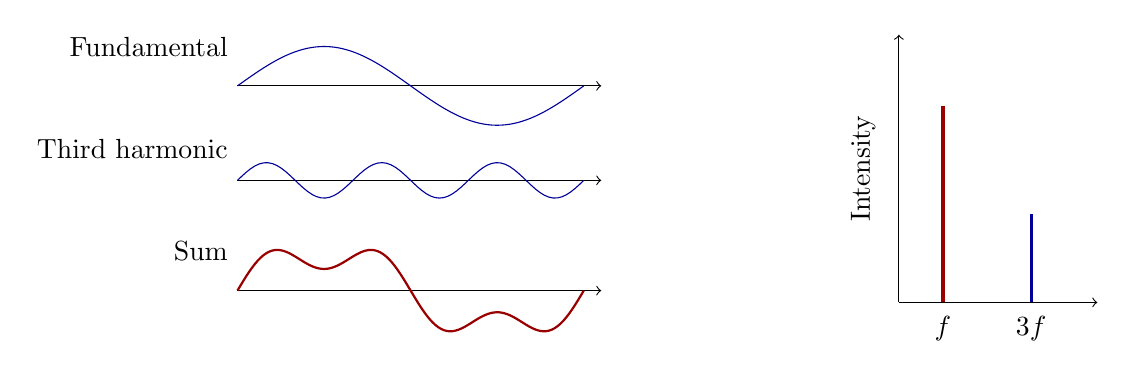
\begin{tikzpicture}[x=0.7cm,y=0.5cm]
  \draw[->] (0,3.6) -- (6.6,3.6);
  \draw[blue!60!black,domain=0:6.283,samples=80] plot (\x,{3.6+1.0*sin(\x r)});
  \node[left] at (0,4.6) {Fundamental};
  \draw[->] (0,1.2) -- (6.6,1.2);
  \draw[blue!60!black,domain=0:6.283,samples=80] plot (\x,{1.2+0.45*sin(3*\x r)});
  \node[left] at (0,2.0) {Third harmonic};
  \draw[->] (0,-1.6) -- (6.6,-1.6);
  \draw[red!60!black,thick,domain=0:6.283,samples=120] plot (\x,{-1.6+1.0*sin(\x r)+0.45*sin(3*\x r)});
  \node[left] at (0,-0.6) {Sum};
  \begin{scope}[xshift=8.4cm]
    \draw[->] (0,-1.9) -- (0,4.9);
    \draw[->] (0,-1.9) -- (3.6,-1.9);
    \draw[red!60!black,very thick] (0.8,-1.9) -- (0.8,3.1);
    \draw[blue!60!black,very thick] (2.4,-1.9) -- (2.4,0.35);
    \node[below] at (0.8,-2.0) {\(f\)};
    \node[below] at (2.4,-2.0) {\(3f\)};
    \node[above,rotate=90] at (-0.25,1.5) {Intensity};
  \end{scope}
\end{tikzpicture}
\caption{A complex waveform is a sum of simple sine waves (left); its spectrum lists the ingredients (right).}
\end{figure}

\begin{challenge}
Shock geometry follows directly. A source moving at \(u>v\) emits wavefronts whose envelope forms a Mach cone with half-angle \(\theta\):

\[
  \sin\theta = \frac{v}{u} = \frac{1}{M},
\]

where \(M=u/v\) is Mach number. Check \(M=1\): \(\theta=90^\circ\), a cone reduced to a flat wall at the threshold of catching one's waves. Greater \(M\) makes a sharper cone. Speedboat wakes, bullet shocks, and aircraft sonic booms share this geometry.

A deeper fact: shorter sounds have broader spectra. Mathematics gives a lower bound on duration \(\Delta t\) times frequency spread \(\Delta f\), of order

\[
  \Delta f\,\Delta t \gtrsim 1 .
\]

A brief click therefore lacks a definite pitch, while a long-ringing tuning fork has a precise one. Note the boundary: this Fourier result applies to every wave and shares mathematics with quantum uncertainty, but the physical origins differ. Quantum uncertainty is not merely caused by waves, but by quantum-state structure. We will recover this thread later.
\end{challenge}

\step{The Model's Limits}

\begin{mainline}
Every useful sound rule has a domain.

First, superposition requires small variations. Ordinary speech and music vary pressure by less than one ten-thousandth of atmospheric pressure, so independent addition works accurately. Near explosions, pressure fluctuations can rival atmospheric pressure itself. Air's elasticity is no longer uniform, profiles deform during travel, and sound speed varies. Shocks inhabit this nonlinear world, where linear acoustics fails altogether.

Second, frequency-independent sound speed is an excellent approximation, not an absolute rule. It works remarkably well in air, giving front- and back-row audiences identical pitch. In solids and many liquids, slight frequency-dependent speeds, dispersion, spread waveforms over long journeys. Seismologists and medical ultrasound practitioners must account for this.

Third, the Doppler formula \(f'=vf/(v-u)\) explicitly requires \(u<v\). At or above sound speed it yields to shock theory. More importantly, do not apply it directly to light. Acoustic Doppler shift is a race relative to a medium; light needs no such track. Its Doppler law must be derived using relativity, similar at low speed and fundamentally different at high speed. That belongs to later chapters.

Fourth, decibels are not purely physical but convert intensity through human hearing's response. Sensitivity also varies greatly with frequency: equal-intensity three-thousand-hertz sound seems much louder than fifty-hertz sound. Loudness is partly physics, partly physiology.

Fifth, sufficiently thin media do not merely weaken sound; they destroy the wave picture. If a molecule typically travels farther than a wavelength before another collision, the local compression relay cannot organize, and there is no sound wave. The upper atmosphere and interstellar space fall into this category.

Common misuses: louder means faster, wrong, amplitude does not change speed. Loud sound travels farther only because more energy takes longer distance to fade below audibility. Higher pitch means harsher and more energetic, wrong, pitch and loudness are independent. Sound in vacuum is very quiet, wrong, it does not exist; this is existence, not degree. Downwind sound is carried by wind, also the wrong picture. Wind is far slower than sound and cannot carry it as a parcel. Typically stronger wind aloft advances the upper wavefront more, bending it toward the ground and extending audible range. This is refraction, not courier delivery.
\end{mainline}

\step{Explaining the Opening Phenomenon}

\begin{mainline}
Return to the poor speaker diaphragm.

First comes superposition in air. Dozens of instruments launch their own compression waves, but at your ear pressure has one value at each instant. All contributions add into one time-varying curve. An entire symphony is, to air, one graph of pressure against time. One membrane suffices because it need not do dozens of things simultaneously: it merely occupies the right position each instant, faithfully replaying the total curve. Prediction 3 is settled: recordings store not instrument lists but samples of this curve at tiny intervals, commonly 44,100 values per second. Playback turns those values back into membrane positions, reviving the curve.

The second step happens in your head. How do you separate drums, guitar, and voice from one tangled eardrum curve? The cochlea contains a basilar membrane, narrow and stiff at its high-frequency end, broad and flexible at its low-frequency end. Different frequencies resonate at different locations and stimulate different nerves, physically performing spectral analysis. It resembles a spectrum analyzer by separating and reporting components. It differs in finite resolution: nearby frequencies mask one another, and the brain then uses experience to reconstruct violin or familiar voice. Formats such as MP3 exploit masking, deleting spectral components hidden by stronger sounds. Files shrink to a tenth with little audible difference. This unexpected third layer makes clear hearing itself a relay between physical analysis and physiological inference.

Information now emerges. Sound conveys identity, words, and mood because the pressure curve can take one of countless shapes. More distinguishable variations permit more messages and information. Vocal cords and tongue write meaning into the waveform, air transmits, and cochlea and brain read. Writing, transmitting, and reading are communication's three stages. Pumping out bell-jar air removes transmission, silencing the alarm. Loud and soft speech use the same medium and relay speed, so arrive together. Equal time wins prediction 2.

This viewpoint explains innumerable applications. Telephones turn waveforms into electrical currents and back. Speech recognition delegates reading to computers. Parking sensors and sonar emit sound and time echoes for range, like bats. Medical ultrasound images the body with inaudible high-frequency sound. Active noise cancellation reverses superposition: measure noise, generate its opposite waveform in real time, and add the two to subtract noise. Concert-hall designers balance reflected sound reaching rear seats against echoes lasting so long that successive notes blur. Wall, seat, and ceiling materials and angles negotiate those echo delays.

The deepest consequence lies in sound's greatest limit. Needing a medium, sound cannot leave the atmosphere. Astronauts facing each other on the Moon cannot hear even shouted voices; they communicate by radio. Radio waves carry waveforms and modulated information like sound but need no medium. What vibrates in a medium-free wave? That question leads from mechanical oscillation to a new concept, the field, beginning the next part on electricity and magnetism, and underlying phones, broadcasting, Wi-Fi, and light.
\end{mainline}

\step{Thought Experiments and Challenges}

\begin{thought}[What If Interstellar Space Were Full of Air?]
The Sun's surface continually vibrates. Astronomers even diagnose its interior from surface motions, a discipline called asteroseismology. Suppose the space between Sun and Earth contained air as dense as at ground level. What would happen?

First, time. Sunlight takes about eight minutes. Sound at 340 meters per second would take about fourteen thousand years to cross the same 150 million kilometers. A mythical herald announcing sunrise by voice would still have the message en route, with over ten thousand years left to wait.

Next, loudness. Intensity falls with distance squared, and the Sun--Earth distance is astronomical. However loudly the Sun shouted, it would fade below audibility here. Real interstellar space is nearly vacuum, so even that attenuating path does not exist.

The thought experiment gives two conclusions. Bad news: the universe's sound is permanently muted; even spectacular stellar explosions send no audible sound. Good news: we can still see the vibration. Solar surface motion changes emitted light, which carries an indirect record of the Sun's voice. Where sound cannot reach, light can. Why? That invaluable question is answered in the next part.
\end{thought}

\begin{puzzles}
\item During a storm, six seconds between lightning and thunder suggest two kilometers. A friend asks whether sound speed really is 340 meters per second. Can it vary, what affects it, and when would your estimate be appreciably wrong? (Hint: recall which medium properties set speed; compare winter and summer, mountain foot and summit. Why can light's travel time be safely neglected?)

\item Why does gently pinching a string telephone's midpoint immediately interrupt it? Could attaching a third cup firmly there create a three-way call, and what happens to volume? (Hint: energy follows vibration. Is the pinched point free to move? How must energy divide when another path is added?)

\item An ambulance travels at thirty meters per second, about 110 kilometers per hour, with a five-hundred-hertz siren. At sound speed 340 meters per second, calculate approaching and receding frequencies. Check that zero vehicle speed recovers five hundred hertz and approach gives higher frequency than recession. (Hint: substitute into \(f'=vf/(v-u)\), making \(u\) negative for recession. Checks are not rituals: explain what failure of each would reveal.)

\item A hammer strike on a table gives a pitchless click; striking a tuning fork gives a sustained precise note. Both arise from vibration, so why does only one have clear pitch? (Hint: frequency precision relates to duration through \(\Delta f\,\Delta t\gtrsim 1\). If this applies to all waves, what does it imply for microscopic waves we will meet later?)
\end{puzzles}
